\documentclass[a4paper,14pt]{article}
%%%%%%%%%%%%%%%%%%%%%%%  ПАКЕТЫ  %%%%%%%%%%%%%%%%%%%%%%%%%%%%%%%%%%%%%%%%%%%%%%
\usepackage{cmap}                               % Чтобы в PDF работал человеческий поиск
\usepackage[X2,T2A]{fontenc}                    % T2A = русская кодировка. X2 = яти
\usepackage[utf8]{inputenc}                     % Ввод в универсальной кодировке
\usepackage{setspace,soulutf8}      		        % Чтобы можно было менять межстрочный и межбуквенный интервалы
\usepackage{amsmath,amsfonts,amssymb,amsthm}    % Символы для математики
\usepackage{mathrsfs}                           % Символы для математики
\usepackage{dsfont}                             % Шрифт для полей действительных, комплексных... чисел командой \mathds
\usepackage[subfigure]{tocloft}  % Многоточие в оглавлении
\usepackage{array,multicol,multirow,bigstrut}   % Чтобы можно было делать в таблице колонки фиксированной ширины, слитные ячейки, вставлять strut'ы.
\usepackage{indentfirst}                        % Абзацный отступ везде
\usepackage[british,russian]{babel}             % Русские переносы, тире, типографика, самодержавие, духовность!
\usepackage[perpage]{footmisc}                  % Сброс счётчика сносок на каждой странице
\usepackage[pdftex,unicode,bookmarks=true,bookmarksopen=true,colorlinks=true,linkcolor=blue,urlcolor=blue,citecolor=blue]{hyperref} % Синие ссылки в PDF
\usepackage{microtype}                          % Свешивающаяся пунктуация и подгонка белого пространства по правилу \pm 2 процента
\usepackage{textcomp}                           % Чтобы в формулах можно было русские буквы писать через \text{}
\usepackage[paper=a4paper,top=12.7mm, bottom=12.7mm,left=12.7mm,right=12.7mm,bindingoffset=6.6mm,includefoot]{geometry} % Достаточно экономные размеры листа и поля для нумерации страниц внизу (для колонтитулов в стиле лекций по матану, нужно includefoot заменить на includehead и не только
\usepackage{xcolor}                             % Чтобы можно было цветные объекты вставлять
\usepackage[pdftex]{graphicx}                   % Чтобы вставились изображения
\usepackage{float,longtable}                    % Поддержка плавающих таблиц и рисунков
\usepackage[margin=0pt,font=small,labelfont=bf,labelsep=period]{caption} % Подписи таблиц и рисунком мелкие, жирные, с принятым в русской типографике разделителем.
\usepackage{rotating}                           % Создание своих акцентов, поворот объекта.
\usepackage{datetime}                           % Отображение времени
%\usepackage{embedfile}                         % Чтобы код LaTeXа включился как приложение в PDF-файл
\usepackage{xspace}
\usepackage{wrapfig,enumitem}                   % Обтекаемые текстом рисунки
\usepackage{mathtools}                          % В тексте используется smashoperator, чтобы избежать некрасивых пробелов вокруг сумм и пределов с большим подстрочником
\usepackage{cancel}                             % Красивое <<вычёркивание>> сокращающихся выражений одноимённой командой
\usepackage{tikz,pgfplots}			% Рисование графиков непосредственно кодом
\usepackage{subfigure}
\usepackage{fancyhdr}	% Пакет для создания колонтитулов в стиле лекций по матану
\usepackage{accents}
\usepackage{pb-diagram}

%%%%%%%%%%%%%%%%%%%%%%%  ПАРАМЕТРЫ  %%%%%%%%%%%%%%%%%%%%%%%%%%%%%%%%%%%%%%%%%%%
\setstretch{1}                          % Межстрочный интервал
\flushbottom                            % Эта команда заставляет LaTeX чуть растягивать строки, чтобы получить идеально прямоугольную страницу
\righthyphenmin=2                       % Разрешение переноса двух и более символов
\pagestyle{plain}                       % Нумерация страниц снизу по центру.
\settimeformat{hhmmsstime}              % Формат времени с секундами
\widowpenalty=300                       % Небольшое наказание за вдовствующую строку (одна строка абзаца на этой странице, остальное --- на следующей)
\clubpenalty=3000                       % Приличное наказание за сиротствующую строку (омерзительно висящая одинокая строка в начале страницы)
\setlength{\parindent}{1.5em}           % Красная строка.
\setlength{\topsep}{0pt}                % Уничтожение верхнего отступа, если он где проявится
%%%%%%%%%%%%%%%%%%%%%%%%%%%%%%%%%%%%%%%%%%%%%%%%%%%%%%%%%%%%%%%%%%%%%%%%%%%%%%%

%%%% Техническая подготовка для определения следующих команд %%%%
\makeatletter
\newcommand*{\relrelbarsep}{.386ex}
\newcommand*{\relrelbar}{%
  \mathrel{%
    \mathpalette\@relrelbar\relrelbarsep
  }%
}
\newcommand*{\@relrelbar}[2]{%
  \raise#2\hbox to 0pt{$\m@th#1\relbar$\hss}%
  \lower#2\hbox{$\m@th#1\relbar$}%
}
\providecommand*{\rightrightarrowsfill@}{%
  \arrowfill@\relrelbar\relrelbar\rightrightarrows
}
\providecommand*{\leftleftarrowsfill@}{%
  \arrowfill@\leftleftarrows\relrelbar\relrelbar
}
\providecommand*{\xrightrightarrows}[2][]{%
  \ext@arrow 0359\rightrightarrowsfill@{#1}{#2}%
}
\providecommand*{\xleftleftarrows}[2][]{%
  \ext@arrow 3095\leftleftarrowsfill@{#1}{#2}%
}
\makeatother



%%%%%%%%%%%%%%%%%%%%% Команды-сокращения %%%%%%%%%%%%%%%%%%%%%%%%%%%%%%%%%%%%%%
\newcommand{\pau}{\hskip .75em plus.1em minus.08em\relax}	% пробел для выражений с кванторами, например «\forall\ \e>0\pau\exists\ \delta\colon», где \e определяется как
\newcommand{\ds}{\displaystyle}			% Быстрое переключение на выключный стиль формулы, где интегралы и суммы большие
\newcommand{\e}{\varepsilon}                % эпсилон
\newcommand{\p}{\partial}                   % частная производная
\renewcommand{\phi}{\varphi}                % Чтоб фи писалась в соответствии с русской традицией
\newcommand{\q}{\varnothing}			% Пустое множество в русской традиции
\newcommand{\N}{\mathds{N}}			% Натуральные числа
\newcommand{\Z}{\mathds{Z}}			% Целые числа
\newcommand{\Q}{\mathds{Q}}			% Рациональные числа
\newcommand{\R}{\mathds{R}}			% Действительные числа
\renewcommand{\C}{\mathds{C}}			% Комплексные числа
\newcommand{\T}{\mathbb{T}}			% Отмеченное разбиение (для интегральных сумм Римана или Римана"--~Стилтьеса
\newcommand{\Rim}{\mathcal R}			% Риман
\renewcommand{\le}{\leqslant}           % Правильное меньше или равно
\renewcommand{\leq}{\leqslant}           % Правильное меньше или равно
\renewcommand{\ge}{\geqslant}           % Правильное больше или равно
\renewcommand{\geq}{\geqslant}           % Правильное больше или равно
\newcommand{\dd}{\setminus}		% Ассоциируется с diagdown, но это именно вычитание множеств
\renewcommand{\iff}{\,\Leftrightarrow\,}	% Если и только если
\newcommand{\imp}{\hspace{1pt plus1pt}\Rightarrow\hspace{1pt plus1pt}}		% Следовательно
\def\hm#1{#1\nobreak\discretionary{}{\hbox{$#1$}}{}} % Команда для переноса на следующую строку символов бинарных операций
\renewcommand{\a}{\langle} 		% Открывающая треугольная скобка
\newcommand{\s}{\rangle}		% Закрывающая треугольная скобка
\newcommand{\ol}[1]{\overline{#1}}	% Надчёркивание аргумента по всей ширине

%%%% СТРЕЛКИ %%%%%%%%%%%%%%
\renewcommand{\to}{\rightarrow}                   % Правильная стрелка вправо («стремится») без возможности подписать
\newcommand{\To}[1]{\xrightarrow{#1}}		% Стрелка «стремится», ширина которой зависит от ширины агрумента-подписи (подпись ставится вверху)
\newcommand{\tend}[1]{\xrightarrow[#1]{}}	% Стрелка «стремится», ширина которой зависит от ширины агрумента-подписи (подпись ставится внизу)
\newcommand{\Tot}[1]{\xrightarrow{\text{#1}}}	% Стрелка «стремится», ширина которой зависит от ширины текстового агрумента-подписи (подпись ставится вверху)
\newcommand{\te}[1][]{\xrightarrow[n\to\infty]{#1}}	% Стремится при n стремящемся к бесконечности
\newcommand{\TE}{\xrightarrow[N\to\infty]{}}	% Стремится при N стремящемся к бесконечности
\newcommand{\neV}{\overline{\vphantom{<}\quad}\kern-.35em\searrow}	% Не возрастает в стиле лекций по анализу
\newcommand{\neU}{\underline{\vphantom{<}\quad}\kern-.35em\nearrow}	% Не убывает
\newcommand{\rsh}[2][P]{\xrightrightarrows[{#2\to\infty}]{#1}}		% Двойная растяжимая стрелка «равномерно сходится последовательность». Снизу стрелки подпись-обязательный-аргумент, к которому приписывается автоматически стремление к бесконечности. Необязательные аргумент изменяет подпись сверху с P на то, что напишите
\newcommand{\rsH}[2][X]{\xrightrightarrows[{#2}]{#1}} % Равномерная сходимость по параметру. Подпись снизу задаётся явно и обязательно; подпись сверху задаётся необязательно, по умолчанию X
\newcommand{\nsh}[2][n]{\xrightarrow[#1\to\infty]{\|\ \|_{#2}}}		% Растяжимая стрелка «сходится по норме». Вид нормы подписывается в обязательном аргументе (например l_2). Необязательный аргумент «что стремится к бесконечности» (стремление к бесконечности приписывается автоматически)


%%%%% Предел как оператор %%%%%%%%
\newcommand{\yo}[2]{\lim\limits_{#1\to#2}}	% предел{при этой букве}{стремящейся сюда}
\newcommand{\prb}[1]{\lim\limits_{#1}}		% предел{по такой базе}

%%%%%% O-символика %%%%%%%%%%%%
\newcommand{\oo}{\overline{\overline o}} 		% o-малое без подписей и скобок (две черты сверху ставятся автоматически). Переопределение этой команды изменит вид всех надстроек, указанных ниже
\newcommand{\ou}{\underline{\underline{O}}}		% Аналогично O-большое
\newcommand{\ouu}[2]{\underset{#2\ }\ou(#1)}		% O-большое{по отношению к чему}{при каком процессе}
\newcommand{\ooo}[2]{\underset{#2\ }\oo(#1)} % o-малое{по отношению к чему}{при каком процессе}
\newcommand{\ooob}[2]{\underset{#2}{\oo\big(#1\big)}}	% Аналогично, только скобки вокруг первого аргумента с плавающим размером
\newcommand{\ooog}[2]{\underset{#2}{\ou\big(#1\big)}}

%%%%%% Дифференцирование %%%%%%%%%%%%%%
\newcommand{\CP}[2]{\frac{\partial #1}{\partial #2}}	% Частная производная{чего}{по чему}
\newcommand{\cP}[2]{\frac{d #1}{d #2}}			% Полная/материальная производная
\newcommand{\Jacoby}[4]{\begin{pmatrix}
\CP {{#1}_{1}}{{#2}_1} 	& \CP{{#1}_{1}}{{#2}_2} & \dots & \CP{{#1}_{1}}{{#2}_{#3}} \\[1ex]
\CP {{#1}_{2}}{{#2}_1} 	& \CP{{#1}_{2}}{{#2}_2} & \dots & \CP{{#1}_{2}}{{#2}_{#3}} \\
\vdots 			& \vdots		& \ddots& \vdots \\
\CP {{#1}_{#4}}{{#2}_1} & \CP{{#1}_{#4}}{{#2}_2}& \dots & \CP{{#1}_{#4}}{{#2}_{#3}}	
\end{pmatrix}}% матрица Якоби{чего}{по чему}{размерность образа}{размерность аргумента}


\newcommand{\ttilde}[1]{\tilde{\tilde{#1}}}	% Набрать символ(ы)-аргумент с двумя узкими волнами
\newcommand{\Til}[1]{\widetilde{#1}{} }		% Набрать символ(ы)-аргумент с волной, ширина которой равна ширине аргумента

%%%% ПОСЛЕДОВАТЕЛЬНОСТИ, СУММЫ, ПРОИЗВЕДЕНИЯ %%%%%
\newcommand{\pos}[2][n]{\big\{{#2}_{#1}\big\}_{#1=1}^\infty} 		% Последовательность: в фигурных скобках аргумент с нижним индексом по умолчанию n; справа от скобок подпись n (или необязательный аргумент) от 1 до бесконечности
\newcommand{\ar}[4]{\big\{{#1}_{#2}\big\}_{#2=#3}^{#4}} % Задание последовательности четырьмя аргументами: что, каким символом нумеруется, откуда, докуда
\newcommand{\Har}[4]{\left\{{#1}_{#2}\right\}_{#2=#3}^{#4}} % Аналог предыдущего, но размер фигурных скобок подстраивается под внутренность.
\newcommand{\AR}[3]{\big\{#1\big\}_{#2}^{#3}} 		% Последовательность. Три аргумента: {что и как нумеруеся}{номер=начальное значение}{конечное значение номера}
\newcommand{\ry}[3][1]{\sum\limits_{{#3}={#1}}^\infty {#2}_{#3}}	% Ряд[с какого номерая начиная]{чего}{как нумеруется}; по умолчанию с единицы; Например, \ry an
\newcommand{\rY}[2][1]{\sum\limits_{{#2}={#1}}^\infty} % Сумма до бесконечности[с какого номера начать]{символ индекса}; например, \rY n или \rY[0]j
\newcommand{\RY}[3]{\sum\limits_{#1 = #2}^{#3}}		% Сумма{по этому индексу}{от этого значения индекса}{до этого значения индекса}; Например, \RY n1N
\newcommand{\tmy}[3][1]{\prod\limits_{#3=#1}^{\infty}#2_{#3}}	% Бесконечное произведение (от слова times), аналог \ry
\newcommand{\tmY}[2][1]{\prod\limits_{#2=#1}^{\infty}} % аналог \rY
\newcommand{\TMY}[3]{\prod\limits_{#1=#2}^{#3}}		% аналог \RY



%%%%% Окружения для нумерованных перечней
\newenvironment{iItems}{\begin{enumerate}\let\AEtheenumi\theenumi{}\renewcommand{\theenumi}{\roman{enumi}}\renewcommand{\labelenumi}{(\theenumi)}}{\renewcommand{\labelenumi}{\theenumi.}\renewcommand{\theenumi}{\AEtheenumi}\end{enumerate}}	% (i), (ii), ...
\newenvironment{azItems}{\begin{enumerate}\let\AEtheenumi\theenumi{}\renewcommand{\theenumi}{\asbuk{enumi}}\renewcommand{\labelenumi}{(\theenumi)}}{\renewcommand{\labelenumi}{\theenumi.}\renewcommand{\theenumi}{\AEtheenumi}\end{enumerate}}	% (а), (б), ...
\newenvironment{roItems}{\begin{enumerate}\renewcommand{\labelenumi}{(\theenumi)}}{\renewcommand{\labelenumi}{\theenumi.}\end{enumerate}}	% (1), (2), ...
\newenvironment{oItems}{\begin{roItems}\setcounter{enumi}{-1}}{\end{roItems}}	% (0), (1), ...
%%% В КОНЦЕ ФАЙЛА ПРИВЕДЕНЫ КОМАНДЫ, КОТОРЫЕ Я НЕ УСПЕЛ ОПИСАТЬ

%%%%%%%%%%%%%%%%%%%% Операторы в смысле LaTeX %%%%%%%%%%%%%%%%%%%%%%%%%%%%%%%%%
\DeclareMathOperator{\sign}{sgn}	% Знак (перестановки)
\DeclareMathOperator{\sgn}{sgn}		% Сокращённая альтернатива sign
\DeclareMathOperator{\diag}{diag}	% Диагональная матрица
\DeclareMathOperator{\const}{const}	% Константа
\DeclareMathOperator{\rang}{rank}         % Оператор ранга
\DeclareMathOperator{\rank}{rank}	% На любой вкус
\DeclareMathOperator{\diam}{diam}	% Диаметр, например, разбиения
\DeclareMathOperator{\card}{card}	% Мощность множества
\DeclareMathOperator{\osc}{osc}		% Осцилляция	
\DeclareMathOperator{\grad}{grad}	% Градиент
\DeclareMathOperator{\intS}{int}	% Внутренность множества
\DeclareMathOperator{\ext}{ext}		% Внешность множества
\DeclareMathOperator{\supp}{supp}
\DeclareMathOperator{\extr}{extr}


%%%%%%% Математическая экзотика %%%%%
\newcommand{\defequiv}{\mathbin{\vbox{\baselineskip=1.95pt\lineskiplimit=0pt\hbox{.}\hbox{.}\hbox{.}}\hskip-0.3em\equiv}} 		% вертикальное троеточие =, то есть «по определению тождественно»
\newcommand{\rus}[1]{\mbox{\rm{\scriptsize{#1}}}}	% команда убивает зависимость русского текста в формуле от стиля абзаца (но и от стиля формулы тоже). Специально для обозначения левой и правой производных, чтобы  f'_п печаталось с прямой буквой «п» и нельзя было спутать с n
\newcommand{\overcirc}[1]{\accentset{\circ}{#1}}	% круг над символом
\newcommand{\overstar}[1]{\accentset{\bigstar}{#1}}	% звезда над символом

%%%%%%%%%%%%%%%%%%% Глобальные текстовые команды %%%%%%%%%%%%%%%%%%%%%%%%%%%%%%
\newcommand{\ENGs}[1]{\foreignlanguage{british}{#1}} % Переключение правил переноса и прочих правил автооформления на английский язык действует на аргумент
\newcommand{\ENG}{\selectlanguage{british}} % Глобальное переключение (если просто начать писать на другом язык, велика вероятность появления очень больших пробелов или помещения части слова за границу листа
\newcommand{\RUS}{\selectlanguage{russian}}
\newcommand{\fnnsp}{\hspace{-0.4em}} % Знак сноски принято ставить до всех знаков препинания, кроме ! ? ...
% А если есть возможность подвинуть низкий знак препинания под сноску, то для этого Андрей Викторович и придумал \fnnsp
\let\myfootnote\footnote
\renewcommand{\footnote}[1]{\myfootnote{\;#1}} % Сноски Андрея Виторовича

%%%%%%%% Определение разрядки разреженного текста и задание красивых и притом регулируемых многоточий
% Зачем и почему описано в блоге http://kostyrka.ru/blog
\newdimen\ellipsiskern
\setlength{\ellipsiskern}{.1em}
\newdimen\ellipsiskernen
\setlength{\ellipsiskernen}{.2em}
\newcommand{\ldotst}{.\kern\ellipsiskern.\kern\ellipsiskern.}	% вместо ... пишем \ldotst{}
\newcommand{\ldotse}{!\kern\ellipsiskern.\kern\ellipsiskern.}	% вместо !.. пишем \ldotse{}
\newcommand{\ldotsq}{?\kern\ellipsiskern\kern-.11em.\kern\ellipsiskern.}	% вместо ?.. пишем \ldotsq{}
\newcommand{\ldotsten}{.\kern\ellipsiskernen.\kern\ellipsiskernen.}		% аглийское ...
\newcommand{\ldotspen}{.\kern\ellipsiskernen.\kern\ellipsiskernen.\kern\ellipsiskernen\kern.15em.}
\newcommand{\ldotseen}{.\kern\ellipsiskernen.\kern\ellipsiskernen.\kern\ellipsiskernen\kern.15em!}
\newcommand{\ldotsqen}{.\kern\ellipsiskernen.\kern\ellipsiskernen.\kern\ellipsiskernen\kern.067em?}
%%%%%%%%%%%%%%%%%%%%%%%%%%%%%%%%%%%%%%%%%%%%%%%%%%%%%%%%%%%%%%%%%%%%%%%%%%%%%%%



%%%%%%%%%%%%%%%%%%%%%%% ДРУГИЕ ПОЛЕЗНЫЕ КОМАНДЫ БЕЗ КОММЕНТАРИЕВ (ПОКА) %%%%%%%
\newcounter{rad}
\setcounter{rad}{1}
% a_1+a_2+\ldots
	\def\rad#1#2{\ifnum \therad < \the\numexpr(#2 + 1)\relax #1_\therad + \addtocounter{rad}{1} \rad{#1}{#2}\else \ldots \fi \setcounter{rad}{1}}
%a_{N+1}+a_{N+2}+\ldots
	\def\raD#1#2#3{\ifnum \therad < \the\numexpr(#2 + 1)\relax #1_{#3{\therad}} + \addtocounter{rad}{1} \raD{#1}{#2}{#3}\else \ldots \fi \setcounter{rad}{1}}
\def\crad#1#2#3#4{\ifnum \therad < \the\numexpr(#4 + 1)\relax #1{\therad}#3 + \addtocounter{rad}{1} \crad{#1}{#2}{#3}{#4}\else \ldots +#1{#2}#3 \fi \setcounter{rad}{1}}
\def\craD#1#2#3#4#5#6{\ifnum \therad < \the\numexpr(#4 + 1)\relax #1{#5{\therad}#6}#3 + \addtocounter{rad}{1} \craD{#1}{#2}{#3}{#4}{#5}{#6}\else \ldots +#1{#5#2#6}#3  \fi \setcounter{rad}{1}}
%repeat argument #1 #2 times
	\def\tfT#1#2{\ifnum \therad < \the\numexpr(#2 + 1)\relax #1\addtocounter{rad}{1} \tfT{#1}{#2}\else \fi \setcounter{rad}{1}}
\def\dI#1#2#3#4#5#6{\ifnum \therad < \the\numexpr(#6 + 1)\relax {#1}_{\therad}{#3}_{\therad}#5\addtocounter{rad}{1} \dI{#1}{#2}{#3}{#4}{#5}{#6}\else \dots #5{#1}_{#2}{#3}_{#4}\fi \setcounter{rad}{1}}
\def\DI#1#2#3#4#5#6{\ifnum \therad < \the\numexpr(#6 + 1)\relax #1\therad#3\therad#5\addtocounter{rad}{1} \DI{#1}{#2}{#3}{#4}{#5}{#6}\else \dots #5#1#2#3#4\fi \setcounter{rad}{1}}
\def\iSum#1#2#3{\ifnum \therad < #3\relax {#1}_{\therad}{#2}_{\the\numexpr(#3 - \therad + 1)\relax}+ \addtocounter{rad}{1}\iSum{#1}{#2}{#3}\else {#1}_{\therad}{#2}_{1}\fi \setcounter{rad}{1}}
\def\tms#1#2{\ifnum \therad < \the\numexpr(#2 + 1)\relax #1_\therad \ifnum \therad < \the\numexpr(#2)\relax \cdot \else \fi\addtocounter{rad}{1} \tms{#1}{#2}\else \cdots \fi \setcounter{rad}{1}}
\def\ctms#1#2#3#4#5{\ifnum \therad < \the\numexpr(#4 + 1)\relax #1{#2\therad}#3 \ifnum \therad < \the\numexpr(#4)\relax \cdot \else \fi\addtocounter{rad}{1} \ctms{#1}{#2}{#3}{#4}{#5}\else \cdots #1{#2#5}#3\fi \setcounter{rad}{1}}
\newcommand{\cSize}{\footnotesize}
\newcommand{\cmt}[1]{\text{\cSize #1}}
\newcommand{\BIggl}[1]{\left#1\vphantom{\Bigg(\frac12\Bigg)^2}\right.}
\newcommand{\BIggr}[1]{\left.\vphantom{\Bigg(\frac12\Bigg)^2}\right#1}


\usepackage{caption}
\usepackage{pdfpages}


\begin{document}
\begin{titlepage}
\thispagestyle{empty}
\setcounter{page}{0}
\begin{center}{
\LargeМосковский государственый университет 

им. М.",В.",Ломоносова

Механико-математический факультет

Кафедра газовой и волновой динамики}
\end{center}
\vspace{120pt}
\begin{center}
\Large Ракитин Виталий Павлович.
\end{center}
\vspace{20pt}
\begin{center}{\LARGE Интегрирование системы ОДУ методом Рунге-Кутта.}
\end{center}

\vspace{80pt}
%\begin{flushleft}
%{\largeНаучный руководитель:

%\vspace{6pt}
%чл.-корр. РАН, проф. Трещев Д.",В.}
%\end{flushleft}
\vfill
\begin{center}
Москва, 2015 год.
\end{center}
\end{titlepage}

\tableofcontents
\newpage

\section{Постановка задачи}

{\bf Задача 2.6: } Решить задачу Коши и построить график траектории движения.
\[
\begin{cases}
	\begin{cases}
	\frac{d^2 x}{dt^2} = y(2 - x^2 - y^2); \\
	\frac{d^2 x}{dt^2} = -x(2 - x^2 - y^2);
    \end{cases}\\
	0 < t < 30; \\
	t = 0: x = 0, y =\alpha, \frac{d x}{dt} =\frac{d y}{dt} = 0;\\
	\alpha \in \{1.0, 0.1\}.
\end{cases}
\]

Данную систему из 2х уравнений второго порядка можно свести к эвкивалентной из 4х уравнений первого порядка. Сделаем замену $\frac{dx}{dt} = u$, $\frac{dy}{dt} = v$, получим
\[
\begin{cases}
	\begin{cases}
	\frac{d x}{d t} = u;\\
	\frac{d y}{d t} = v;\\
	\frac{d u}{d t} = y(2 - x^2 - y^2); \\
	\frac{d v}{d t} = -x(2 - x^2 - y^2);
    \end{cases}\\
	0 < t < 30; \\
	t = 0: x = 0, y =\alpha, u = v = 0;\\
	\alpha \in \{1.0, 0.1\}.
\end{cases}
\]

Так~как данная задача не~имеет аналитического решения, напишем компьютерную программу на~языке программирования~$C$ для~численного решения.

\section{Метод решения}
Для решения данной задачи применим метод Рунге - Кутты 5-го порядка с коэффициентами Дормана-Принса 5(4). Для~этого зафиксируем следующие числа 
\begin{center}
\begin{tabular}{|c|ccccccc|}
\hline
{\bf $\alpha$} & \multicolumn{7}{|c|}{{\bf $\beta$}}\\
\hline
    & & & & & & &\\
$0$ & & & & & & & \\ 
    & & & & & & &\\
$\frac{1}{5}$ &$\frac{1}{5}$ & & & & &  &\\
& & & & & &  &\\
$\frac{3}{10}$ &$\frac{3}{40}$ &$\frac{9}{40}$  & & & &  &\\ 
& & & & & &  &\\
$\frac{4}{5}$ &$\frac{44}{45}$ &$-\frac{56}{15}$  &  $\frac{32}{9}$& & & & \\
& & & & & &  &\\
$\frac{8}{9}$ &$\frac{19372}{6561}$ &$-\frac{25360}{2187}$  &  $\frac{64448}{6561}$& $-\frac{212}{729}$ & & & \\
& & & & & & &\\
$1$ &$\frac{9071}{3168}$ &$-\frac{355}{33}$  &  $\frac{46732}{5247}$& $\frac{49}{176}$ &  $-\frac{5103}{18656}$&  &\\
& & & & & & & \\
$1$ &$\frac{35}{384}$ &$0$  &  $\frac{500}{1113}$& $\frac{125}{192}$ &  $-\frac{2187}{6784}$&$\frac{11}{84}$ & \\
& & & & & & & \\
\hline
& & & & & & & \\
$p$ &$\frac{35}{384}$ &$0$  &  $\frac{500}{1113}$& $\frac{125}{192}$ &  $-\frac{2187}{6784}$&$\frac{11}{84}$ & 0 \\
& & & & & & & \\
\hline
& & & & & & & \\
$\bar p$ &$\frac{5179}{57600}$ &$0$  &  $\frac{7571}{16695}$& $\frac{393}{640}$ &  $-\frac{92097}{339200}$&$\frac{187}{2100}$&$\frac{1}{40}$  \\
& & & & & & & \\
\hline
\end{tabular}
\end{center}

Последовательно получим систему, где $y_n \in \{x_n, y_n, u_n, v_n\}$,
\[
	\begin{cases}
k_1(h) = h f \left(t_n, y_n\right);\\
k_2(h) = h f \left(t_n + \alpha_2 h,y_n+\beta_{21}k_1(h)\right);\\
\dots\\ 
k_q(h) = h f \left(t_n + \alpha_q h,y_n+ \sum\limits_{i=1}^{q-1} \beta_{qi}k_i(h)\right).\\
	\end{cases}\\
\]
которая после подставления чисел $\alpha_i,  p_i, \beta_i$ принимает вид
\[
\begin{cases}
k_1(h) = h f \left(t_n,y_n \right);\\
\\
k_2(h) = h f \left(t_n + \frac{1}{5}h,y_n+\frac{1}{4} k_1\right);\\
\\
k_3(h) = h f \left(t_n + \frac{3}{10}h,y_n+\frac{3}{40}k_1 + \frac{9}{40}k_2\right);\\
\\
k_4(h) = h f \left(t_n + \frac{4}{5}h, y_n + \frac{44}{45}k_1 - \frac{56}{15} k_2 + \frac{32}{9} k_3\right);\\
\\
k_5(h) = h f \left(t_n + \frac{8}{9}h,y_n+\frac{19372}{6561}k_1 - \frac{25360}{2187} k_2 +\frac{64448}{6561} k_3 - \frac{212}{729} k_4\right);\\
\\
k_6(h) = h f \left(t_n + h,y_n + \frac{9017}{3168}k_1 - \frac{355}{33}k_2  + \frac{46732}{5247} k_3 + \frac{49}{176} k_4 - \frac{5103}{18656} k_5 \right);\\
\\
k_7(h) = h f \left(t_n + h,y_n + \frac{35}{384}k_1 + \frac{500}{1113} k_3 + \frac{125}{192} k_4 - \frac{2187}{6784} k_5 + \frac{11}{84} k_6 \right).\\

\end{cases}\\
\]

\[
y_{n}(t+h) = y_n (t) + \sum_{i=1}^q {p_ik_i} = y_n (t) + \frac{35}{384}k_1 + \frac{500}{1113} k_3 + \frac{125}{192} k_4 - \frac{2187}{6784} k_5 + \frac{11}{84} k_6;
\]
\[
\bar {y}_{n}(t+h) = y_n (t) + \sum_{i=1}^q {\bar p_ik_i} = y_n (t) + \frac{517}{57600}k_1 + \frac{7571}{16695}k_3 +\frac{393}{640}k_4 - \frac{92097}{339200}k_5 + \frac{187}{2100}k_6 + \frac{1}{40}k_7. 
\]

Таким образом величина погрешности имеет порядок точности $O(h^5)$ и её можно оценить двумя способами. Во-первых, как~расстояние между двумя точками $A$ и $\bar A$
\[
Err = \sqrt{(x_n - \bar x_n)^2 + (y_n - \bar y_n)^2 + (u_n - \bar u_n)^2 + (v_n - \bar v_n)^2}. 
\]
Во-вторых, как максимум расстояний между соответствующими координатами, а именно
\[
Err = \max \left( x_n - \bar x_n,y_n - \bar y_n, u_n - \bar u_n, v_n - \bar v_n \right). 
\]
Для удобства будем использовать второй вариант.
\subsection{Горизонтальная процедура автоматического выбора шага}
Для того, чтобы избешать сильного отклонения от допустимого для корректных вычислений значения шага, напишем так же функцию, которая будет автоматически изменять наш шаг в течении всего времени расчётов.

Пусть $\e$ "--- это заранее заданная точность нашей погрешности $Err$, 
а значения корректирующих констант заданы следующим образом (их можно менять по усмотрению программиста)  
\[
FAC = 0.9, \qquad FACMIN = 0.5,\qquad FACMAX = 2.0.
\]
В таком случае формула для изменения шага будет представлена в следующем виде
\[
h_{new} = h \cdot \min \left(FACMAX, \max \left(FACMIN, \left(\frac{\e}{Err} \right)^{\frac{1}{1 + p}} \right)\right),
\]
где $p = 5$ "--- порядок алгоритма.
Таким образом, при расчётах будем производить коррекцию шага до тех пор, пока не добьёмся нужного порядка погрешности наших вычислений.
\section{Оценка корректности результата}
Прежде всего нам необходимо знать, можем ли мы доверять полученному результату. Для оценки корректности работы программы будем использовать нам необходимо понять, какова погрешность наших измерений. Для этого будем высчитывать два значения:
\begin{enumerate}
\item велечина отклонения на каждом шаге;
\item глобальная велечина отклонения.
\end{enumerate}
\subsection{Оценка локального отклонения (на шаге)}
Оценивать велечину отклонения на каждом шаге не имеет никакого смысла из-за значительного увелечения времени работы программы. Поэтому, для этой оценки проведём все вышеизложенные вычисления для трёх значений точности велечины отклонения, а именно $-7, -9$ и $-11$. Далее зафиксируем 4 момента времени: $\frac{T}{4}, \frac{T}{2}, \frac{3T}{4}, T$, где $T$ "--- полное время работы нашей программы. После этого вычислим все значение переменных в каждой из этих точек, и проверим следующее соотношение
\[
variation = \frac{y_{-11} - y_{-9}}{y_{-9} - y_{-7}} \approx 100^{\frac{s}{s+1}} = 100^{\frac{5}{5+1}} \approx  46.42 
\]

После проведения всех расчётов для $\alpha = 1.0$ были получены следующие величины
\[
\text{При $ t = 0.875 $ для переменной $x$: } \quad variation = 2.115109
\]
\[
\text{При  $t = 0.875 $ для переменной $y$: }\quad variation = 2.337501
\]
\[
\text{При $ t = 0.875 $ для переменной $u$: } \quad variation = 1.943925
\]
\[
\text{При  $t = 0.875 $ для переменной $v$: }\quad variation = 2.170464
\]
\[
\text{При  $t = 1.75$ для переменной $x$: } \quad variation = 1.880996
\]
\[
\text{При  $t = 1.75 $ для переменной $y$: }\quad variation = 1.996141
\]
\[
\text{При  $t = 1.75$ для переменной $u$: } \quad variation = 1.646851
\]
\[
\text{При  $t = 1.75 $ для переменной $v$: }\quad variation = 1.792992
\]
\[
\text{При  $t = 2.625 $ для переменной $x$: }\quad variation = 1.194104
\]
\[
\text{При  $t = 2.625 $ для переменной $y$: }\quad variation = 1.057303
\]
\[
\text{При  $t = 2.625 $ для переменной $u$: }\quad variation = 1.490886
\]
\[
\text{При  $t = 2.625 $ для переменной $v$: }\quad variation = 1.573281
\]
\[
\text{При  $t = 3.5 $ для переменной $x$: }\quad variation =  83.63506
\]
\[
\text{При  $t = 3.5 $ для переменной $y$: } \quad variation = 1.837813
\]
\[
\text{При  $t = 3.5 $ для переменной $u$: }\quad variation =  6.108553
\]
\[
\text{При  $t = 3.5 $ для переменной $v$: } \quad variation = 1.147372
\]

\subsection{Оценка глобальной погрешности.}
Для вычисления глобальной погрешности введём множество переменных $\delta_i:$ 
\[
 \delta_0 = 0, \qquad \delta_{k+1} = Err_{k} + \delta_{k} \cdot e^{\int\limits_{t_k}^{t_{k+1}} \mu(s) ds} 
\]
Интеграл в предыдущем выражении можно приблизить следующим образом
\[
\int\limits_{t_k}^{t_{k+1}} \mu(s) ds = (t_{k+1} - t_k) \cdot Hmax \left(\frac{J + J^T}{2} \right),
\]
где $J$ "--- матрица Якоби исходной системы дифференциальных уравнений, а $Hmax$ "--- функция, возвращающая максимальное собственное значение полученной матрицы. 

\[
J =
\left(
\begin{array}{cccc}
 0 & 0 & 1 & 0 \\
 0 & 0 & 0 & 1 \\
 -2 x y & -x^2-3 y^2+2 & 0 & 0 \\
 3 x^2+y^2-2 & 2 x y & 0 & 0 \\
\end{array}
\right)
\]
Соответственно, 
\[
A = \frac{J + J^T}{2} = 
\left(
\begin{array}{cccc}
 0 & 0 & \frac{1}{2} (1-2 x y) & \frac{1}{2} \left(3 x^2+y^2-2\right) \\
 0 & 0 & \frac{1}{2} \left(-x^2-3 y^2+2\right) & \frac{1}{2} (2 x y+1) \\
 \frac{1}{2} (1-2 x y) & \frac{1}{2} \left(-x^2-3 y^2+2\right) & 0 & 0 \\
 \frac{1}{2} \left(3 x^2+y^2-2\right) & \frac{1}{2} (2 x y+1) & 0 & 0 \\
\end{array}
\right)
\]
Тогда собственные значения матрицы $A$ будут выражаться в следующем виде
\[
\lambda_1 = -x^2-y^2-\sqrt{4 x^4+8 x^2 y^2-8 x^2+4 y^4-8 y^2+5}, \qquad \lambda_2 = x^2+y^2-\sqrt{4 x^4+8 x^2 y^2-8 x^2+4 y^4-8 y^2+5}
\]
\[
\lambda_3 =-x^2-y^2+\sqrt{4 x^4+8 x^2 y^2-8 x^2+4 y^4-8 y^2+5}, \qquad \lambda_4 = x^2+y^2 +\sqrt{4 x^4+8 x^2 y^2-8 x^2+4 y^4-8 y^2+5}.
\]
Несложно заметить, что максимальным собственным значением является именно $\lambda_4$, которое и будем использовать в дальнейших расчётах. Так же вспомним, что $ t_{k+1} - t_k = h$. Значит окончательные формулы для расчёта погрешности принимают вид
\[
\delta_0 = 0, \qquad\delta_{k+1} = Err_{k} + \delta_{k} \cdot e^{\lambda}, \qquad \lambda = \int\limits_{t_k}^{t_{k+1}} \mu(s) ds = h \cdot \left(x^2+y^2 +\sqrt{4 x^4+8 x^2 y^2-8 x^2+4 y^4-8 y^2+5} \right).
\]

\section{Результаты}
По вышеописанному алгоритму была написана компьютерная программа на языке программирования $C$. По результатам её работы было получено множество точек, составляющих траекторию движения системы, описанной данными уравениями.
Однако, опытным путём было выяснено, что для $\alpha = 1.0$. при стремлении $t \to 3.6524$ значения скоростей стремяться к бесконечности. Поэтому расчёты производились до предельного значения точности шага, который был выбран следующим образом $H_{DEFAULT} = 10^{-15}$ и расчёты происходили до соответствующего момента времени $t = 3.5$. После этого по описанному выше алгоритму были посчитаны величины погрешности, которые удовляют всем поставленым ранее ограничениям и указывают на то, что~полученная программа работает корректно.

Так же для проверки данная задача была решена с помощью пакета {\it Wolfram Mathematica 9} (см.~прилож.~\ref{Task1_Wolfram}). Отчётливо видно, что при запуске {\it Wolfram} выдаёт следющую ошибку:

 {\it "At t = 3.652401607212685, step size is effectively zero; singularity or stiff system suspected".}\\
Таким образом, аналагично нашей программе, был произведён анализ до момента времени $t = 3.5$.

Аналогично при $\alpha = 0.1$ критическим значением оказалось $t = 5$.
\subsection{Визуализация полученных результатов}
Для более наглядного представления полученных результатов была написана компьютерная программа на языке программирования $Python$, с помощью библиотеки $Matplotlib$, которая строит графики зависимости наших координат от времени, а так же друг от друга, а именно x(t), y(t) и y(x) (см.~рис.~\ref{py1}). 
Соответствующие графики для $\alpha = 1.0$ представлены на рис.~(\ref{myx-y}),~(\ref{myt-y}),~(\ref{myt-x}) и $\alpha = 0.1$ на ~(\ref{1myx-y}),~(\ref{1myt-y}),~(\ref{1myt-x})

\subsection{Анализ полученных результатов.}
Проведём анализ полученных результатов можно провести в три стадии.
\begin{enumerate}
\item Несложно заметить, что полученное графики полностью совпадают с теми, что полученны с помощью пакета {\it Wolfram Mathematica 9} (см.~прилож.~\ref{Task1_Wolfram} и рис.~(\ref{myx-y}),~(\ref{myt-y})~и~(\ref{myt-x})).
\item Из-за того, что максимальное собственное значение матрицы
\[
A = \frac{J + J^T}{2}
\]
быстро достигает больших значений, то экспонента, а соответственно и велечина глобальной погрешности, растут с крайне высокой скоростью, поэтому через какое-то время они переходят через точную верхнюю гран множества допустим значений соответствующего типа. Это явление делает невозможным подсчёт глобального отклонения. 
\item Из-за того, что значение скорости быстро убегает в бесконечность, количество шагов метода Рунге-Кутта так же слишком мало для~корректного подсчёта локального отклонения.

\begin{figure}[H]
\noindent\centering{
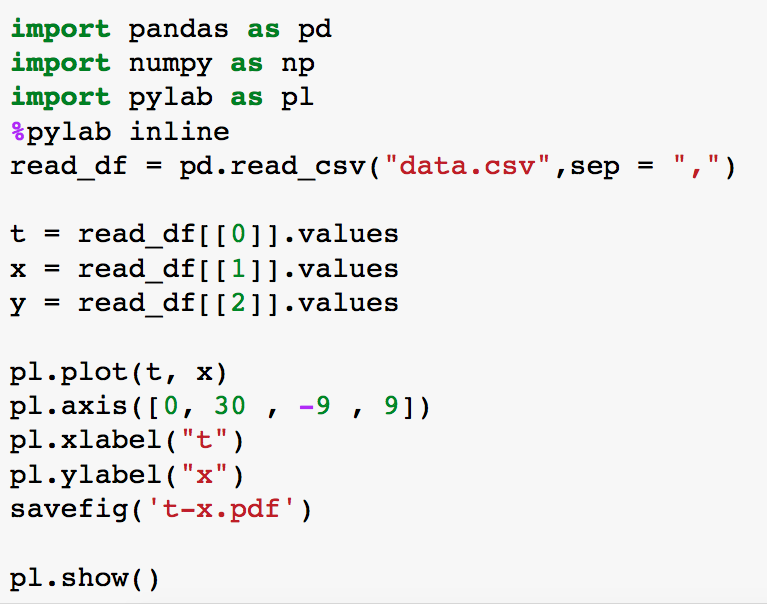
\includegraphics[width=110mm]{pictures/py1.png} 
  \caption{Код на языке $Python$ для построения графика $x(t)$.}
  \label{py1}}
\end{figure}
\begin{figure}[H]
\centering
    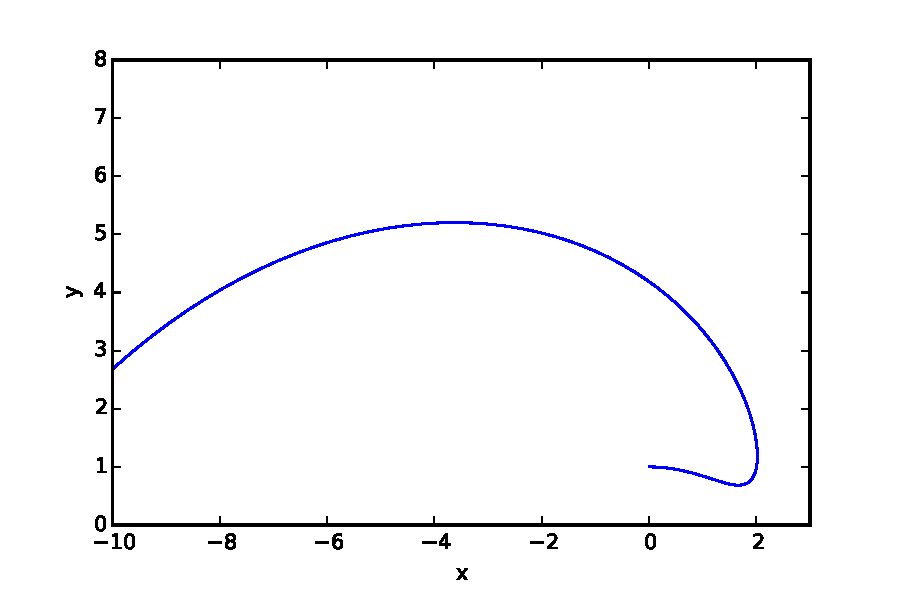
\includegraphics[width=100mm]{pictures/10x-y.pdf}
    \caption{Решение задачи 2.6 при $\alpha = 1.0$. График зависимости $y(x)$}
    \label{myx-y}
\end{figure}
\end{enumerate}
\begin{figure}[H]
\centering
    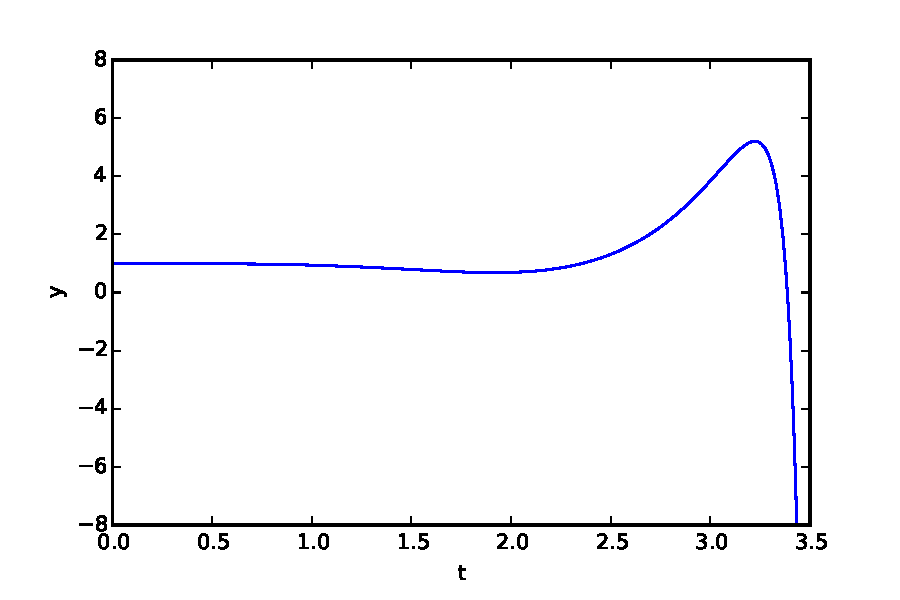
\includegraphics[width=100mm]{pictures/10t-y.pdf}
    \caption{Решение задачи 2.6 при $\alpha = 1.0$. График зависимости $y(t)$}
    \label{myt-y} 
\end{figure}
\begin{figure}[H]
\centering
    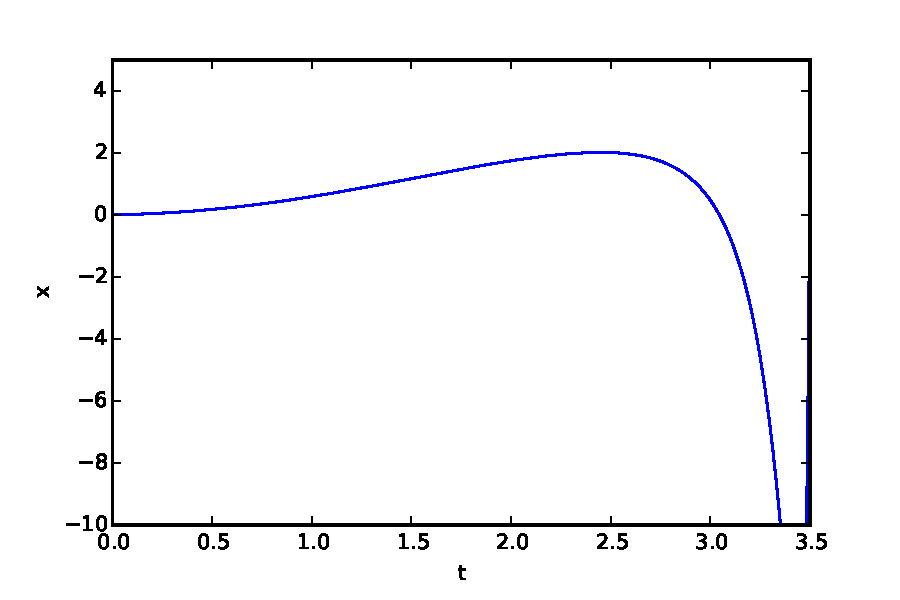
\includegraphics[width=110mm]{pictures/10t-x.pdf}
    \caption{Решение задачи 2.6 при $\alpha = 1.0$. График зависимости $x(t)$}
    \label{myt-x}
\end{figure}
\begin{figure}[H]
\centering
    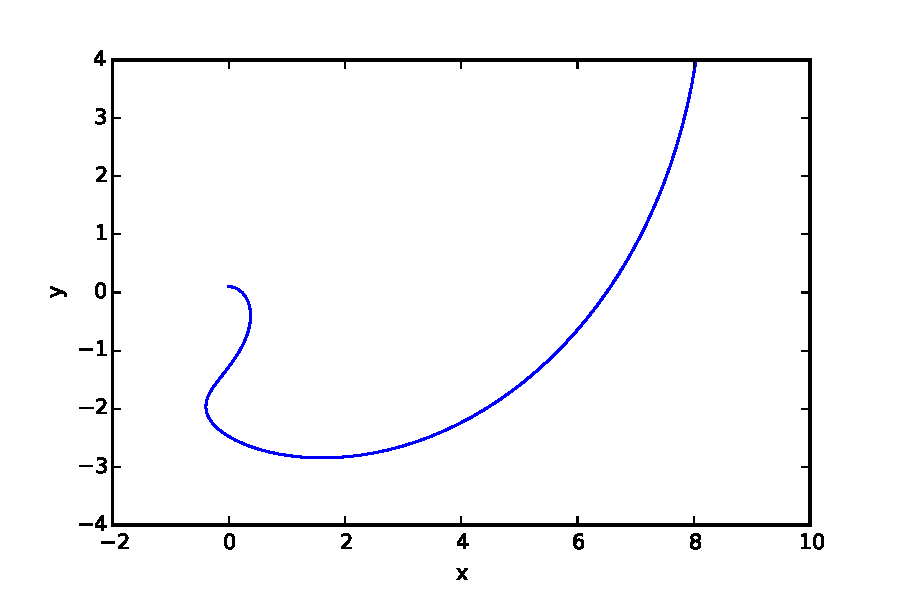
\includegraphics[width=110mm]{pictures/01x-y.pdf}
    \caption{Решение задачи 2.6 при $\alpha = 0.1$. График зависимости $y(x)$}
    \label{1myx-y}
\end{figure}
\begin{figure}[H]
\centering
    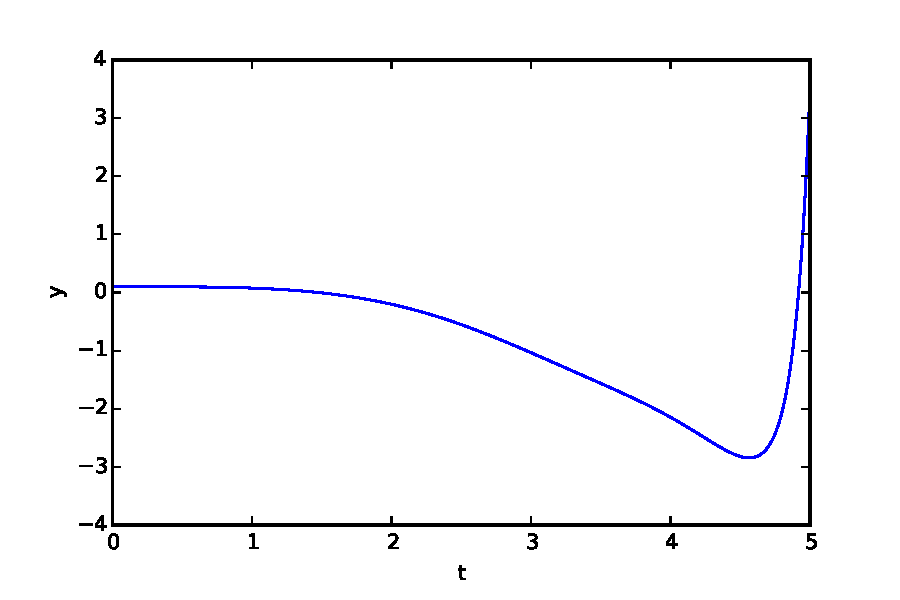
\includegraphics[width=110mm]{pictures/01t-y.pdf}
    \caption{Решение задачи 2.6 при $\alpha = 0.1$. График зависимости $y(t)$}
    \label{1myt-y} 
\end{figure}
\begin{figure}[H]
\centering
    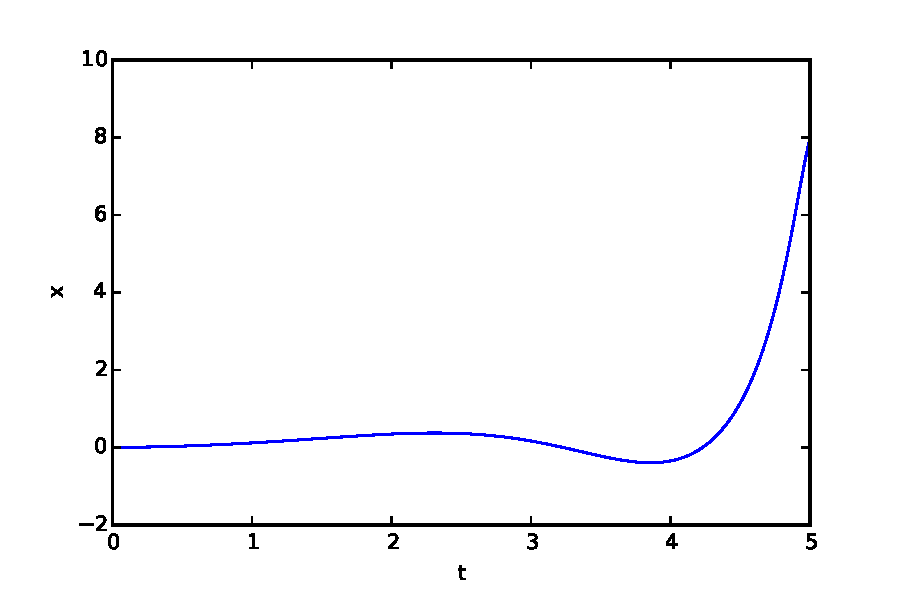
\includegraphics[width=110mm]{pictures/01t-x.pdf}
    \caption{Решение задачи 2.6 при $\alpha = 0.1$. График зависимости $x(t)$}
    \label{1myt-x}
\end{figure}

\section{Гармонический осциллятор}
Дабы отбросить все сомнения в полученных результатах, проверим работоспособность программы на более простом случае с заранее известным решением, а именно на гармоническом осцилляторе
\[
\begin{cases}
	\frac{d x}{d t} = y;\\
	\frac{d y}{d t} = -x;\\
	0 < t < 30; \\
	t = 0: x = 0, y = 8.
\end{cases}
\]

Визуализация численного решения данной задачи с помощью нашей программы представлена в виде графиков на рис.(\ref{t-x}), (\ref{t-y}) и (\ref{x-y}). Для удобства проверки дополнительно решим нашу задачу с помощью пакета {\it Wolfram Mathematica 9} (см.~рис.~\ref{Wolfram}).
Сравнивая полученные результаты можно заметить, что полученные решения абсолютно идентичны, на основе чего можно сделать вывод о корректности работы программы. Однако, для большей достоверности проверим так же численные оценки наших погрешностей.\\
\begin{enumerate}
\item Для вычисления {\bf глобальной погрешности} найдём матрицу Якоби нашей системы
\[
J = \left(
\begin{array}{cc}
 0 & 1 \\
 -1 & 0 \\
\end{array}
\right),
\qquad
A = \frac{J + J^T}{2} =
\left(
\begin{array}{cc}
 0 & 0 \\
 0 & 0 \\
\end{array}
\right)
\]
\[
\lambda_{1,2} = 0, \qquad \delta_0 = 0, \qquad \delta_{k+1} = Err_{k} + \delta_{k}.
\]
Таким образом были получены следюущие значения глобальной погрешности:
\[
\text{для точности погрешности -7-го порядка } \delta_k =  2.433796 \cdot 10^{-6}
\]
\[
\text{для точности погрешности -9-го порядка } \delta_k =  3.964618 \cdot 10^{-7}
\]
\[
\text{для точности погрешности -11-го порядка } \delta_k =  8.135620 \cdot 10^{-9}
\]

\item А оценка {\bf локального отклонения на шаге} для каждой точки $t = \{50, 100, 150, 200\}$ получилась равна в районе $100 \pm 2$.
\end{enumerate}

На основе выше сказанного можно сделать вывод, что полученная программа работает корректно.
\newpage
\begin{figure}[H]
\centering
    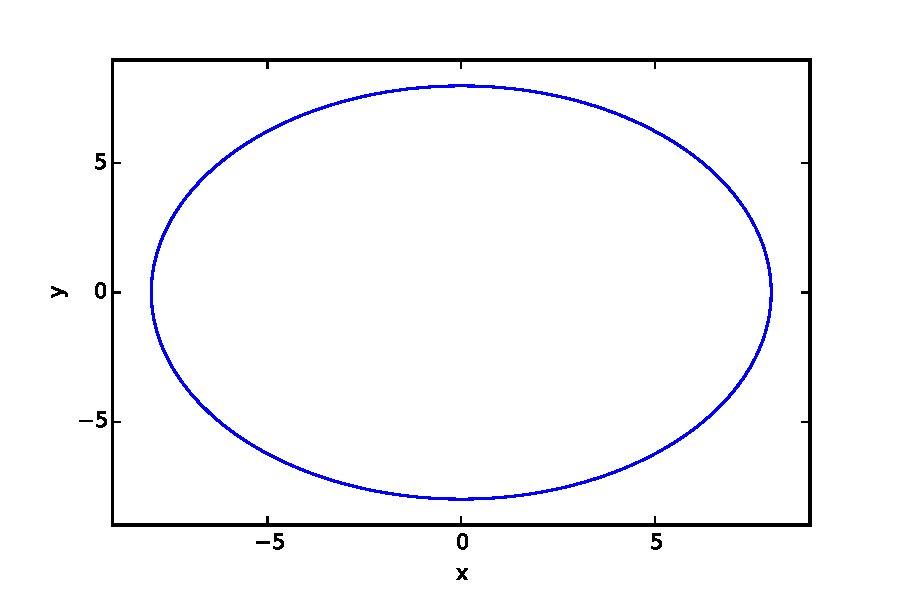
\includegraphics[width=100mm]{pictures/x-y.pdf}
    \caption{Решение задачи о математическом осцилляторе. График зависимости $y(x)$}
    \label{x-y}
\end{figure}
\begin{figure}[H]
\centering
    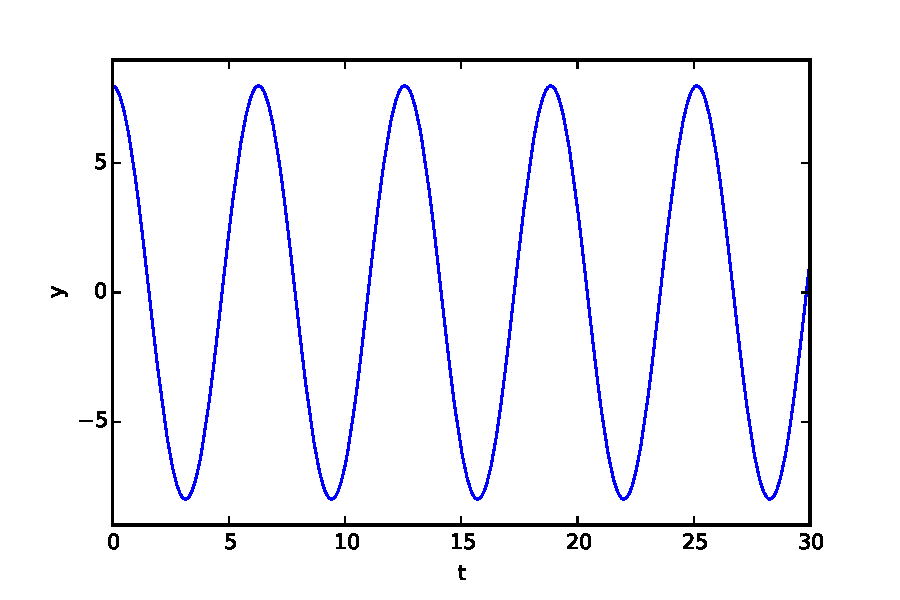
\includegraphics[width=100mm]{pictures/t-y.pdf}
    \caption{Решение задачи о математическом осцилляторе. График зависимости $y(t)$}
    \label{t-y} 
\end{figure}
\begin{figure}[H]
\centering
    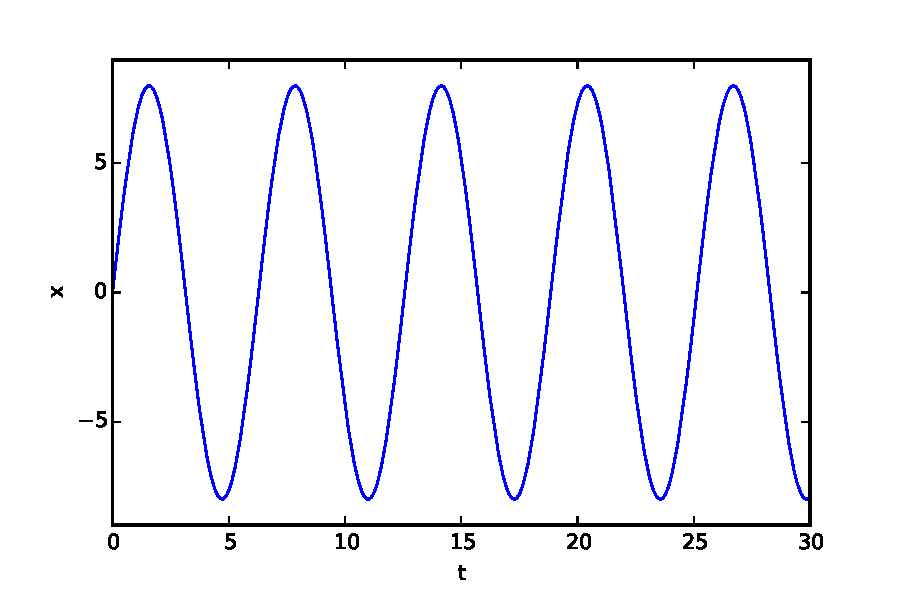
\includegraphics[width=100mm]{pictures/t-x.pdf}
    \caption{Решение задачи о математическом осцилляторе. График зависимости $x(t)$}
    \label{t-x}
\end{figure}

%\begin{figure}[bh]
%\noindent\centering{
%\includegraphics[width=180mm]{oscillator.pdf} 
%  \caption{Решение задачи о математическом осцилляторе в Wolfram Mathematica 9.}
%  \label{Wolfram}}
%\end{figure}

\newpage
\section{Приложения}
\subsection{Решение задачи 2.6 Wolfram Mathematica 9.}
\label{Task1_Wolfram}
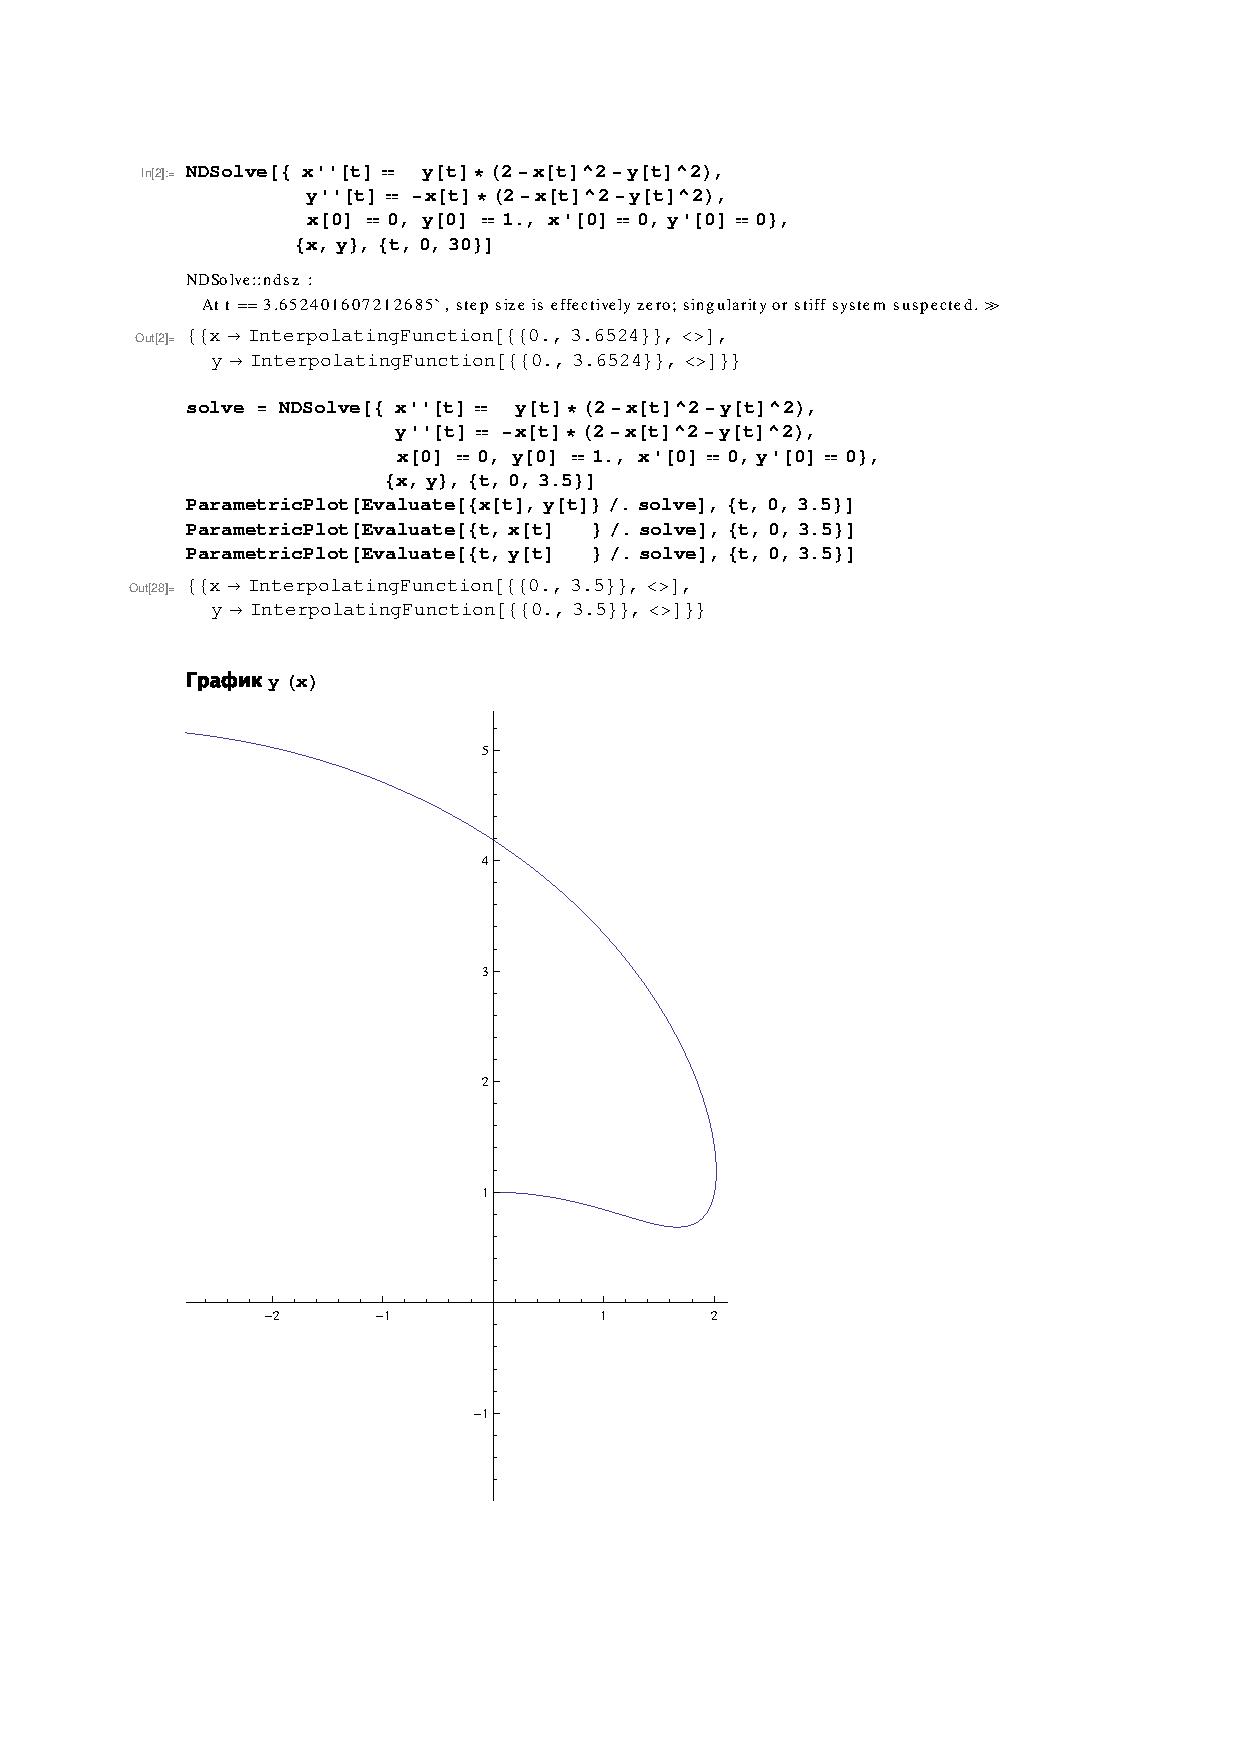
\includepdf[pages={1,2}]{pictures/mytask.pdf}


\subsection{Решение задачи о математическом осцилляторе в Wolfram Mathematica 9.}
\label{Wolfram}
\includepdf[pages={1}]{pictures/oscillator.pdf}


\end{document}